\begin{figure}[t]
  \centering
  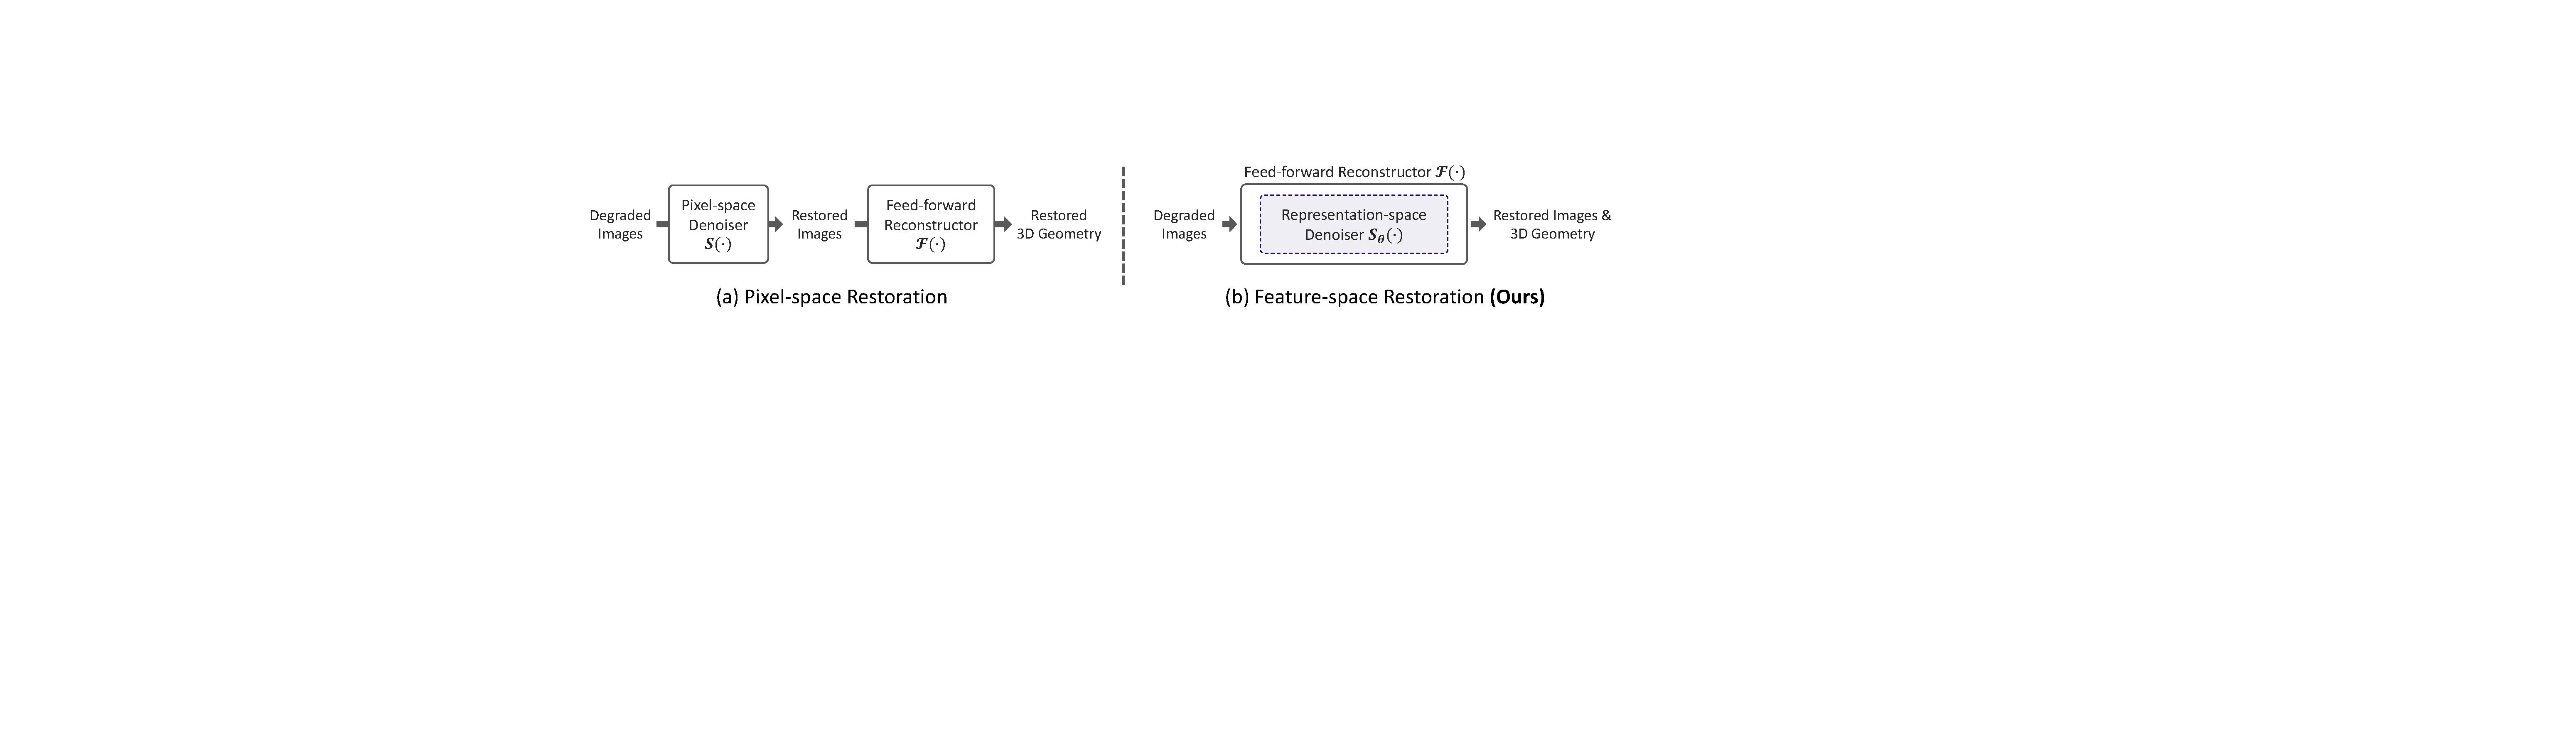
\includegraphics[width=\textwidth]{asset/fig_comparison_copy_2.pdf}
\vspace{-10pt}
\caption{\textbf{Comparison of restoration denoising spaces.}
(a) A {restore-then-reconstruct} pipeline first performs pixel-space restoration prior to 3D reconstruction. However, performing restoration in a single-view setting~\cite{zamir2022restormer, conde2024high, chen2023hierarchical} or within a heavily compressed VAE-based latent space~\cite{mao2025sir, kingma2013auto} fails to preserve cross-view consistency and fine-grained geometric details, which often results in suboptimal geometric reconstruction. (b) In contrast, our \textbf{Geometry-Aware Representation Denoising (GARD)} operates on geometry-aware latent representations within a feed-forward reconstruction model, enabling the joint recovery of restored images and consistent 3D geometry across views.}
\label{fig:comparison}
% \vspace{-10pt}
\end{figure}

\section{Related Work}
\label{sec:rel_work}

% \paragraph{Multi-View 3D Reconstruction.}
% Conventional 3D reconstruction~\cite{hartley2003multiple, schonberger2016structure, Schonberger_2016_CVPR, furukawa2010towards, furukawa2015mvs,SNAVELY-IJCV08, furukawa2010towards} relied on multi-stage pipelines involving keypoint detection~\cite{DBLP:journals/corr/abs-1905-03561,DeTone_2018_CVPR_Workshops, an2024cross} and matching~\cite{4587673, Sun_2021_CVPR, Edstedt_2024_CVPR}, triangulation~\cite{sturmrichard}, and Structure from Motion (SfM) followed by multi-view stereo (MVS). Although effective, their multi-stage design introduces complex optimization, error accumulation, and limited scalability. Recently, feed-forward reconstruction models such as DUSt3R~\cite{wang2024dust3r}, MASt3R~\cite{leroy2024grounding}, 
% VGGT~\cite{wang2025vggt}, and DepthAnything3~\cite{depthanything3} have demonstrated that 3D reconstruction can be addressed using standard transformer backbones~\cite{vaswani2017attention, dosovitskiy2020image} trained on large-scale data, without requiring task-specific geometric pipelines. These approaches infer scene geometry from multi-view inputs in a single forward pass, drastically simplifying reconstruction and enabling strong generalization. Their success highlights a broader insight: beyond architectural complexity, the quality of the underlying visual representation is often a primary determinant of reconstruction performance. However, because these models infer geometry directly from visual features, they are inherently sensitive to input degradations that corrupt those features, motivating the need for restoration methods that are aware of and compatible with their geometry-aware representation spaces.


% \paragraph{Multi-view Image Restoration.}
% Image restoration~\cite{Jiang_2025, chen2026lovif2026challengerealworld, zamir2022restormer, Youk_2024_CVPR, zuo2018convolutional, nah2018deepmultiscaleconvolutionalneural} aims to recover a clean image from degraded observations, encompassing tasks such as deblurring~\cite{liang2024vrt, zamir2022restormer, chen2023hierarchical}, denoising~\cite{zamir2022restormer, zhang2018ffdnet, zamfir2024complexityexperts}, and super-resolution~\cite{lin2024diffbir, duan2025dit4sr, min2025text, kim2025unifieddiffusiontransformerhighfidelity}. Early CNN-based methods~\cite{zuo2018convolutional, zhang2018ffdnet} were followed by transformer architectures~\cite{zamir2022restormer, chen2023hierarchical} that capture long-range dependencies, with Restormer~\cite{zamir2022restormer} and Hi-Diff~\cite{chen2023hierarchical} achieving strong benchmark results. Separately, InstructIR~\cite{conde2024high} conditions restoration on natural language prompts to handle multiple degradation types within a single model. However, these methods are designed for single-image restoration and thus cannot enforce cross-view geometric consistency, which is critical for multi-view reconstruction. While SIR-Diff~\cite{mao2025sir} leverages a diffusion model for restoration, it relies on VAE-based latent spaces~\cite{kingma2013auto}, where feature compression limits fine-grained detail and geometric fidelity. This highlights a key limitation: image-space methods lack consistency, while compressed latent spaces lose information. These challenges motivate restoring in a representation that is both expressive and geometry-aware, enabling consistent and detail-preserving recovery for multi-view 3D reconstruction.

\paragraph{Robust multi-view 3D reconstruction.}
The advent of feed-forward 3D reconstruction models~\cite{wang2024dust3r, leroy2024grounding, wang2025vggt, wang2025pi, depthanything3} has substantially advanced the field of multi-view 3D reconstruction. These models enable direct inference of scene geometry from multi-view images in a single forward pass, effectively replacing conventional multi-stage optimization pipelines~\cite{hartley2003multiple, schonberger2016structure, Schonberger_2016_CVPR, furukawa2010towards, furukawa2015mvs, DeTone_2018_CVPR_Workshops, an2024cross, 4587673, Sun_2021_CVPR}. Nevertheless, their performance degrades significantly in real-world settings~\cite{nah2017deep, rim2020real, malyugina2025unsupervised, liu2024boosting, han2025emergent}, where observations often contain noise such as distractors and degradations, since these models are primarily trained under ideal conditions with clean inputs. Prior works~\cite{han2025emergent, panvisual} have addressed robust multi-view 3D reconstruction in the presence of distractors. For example, RobustVGGT~\cite{han2025emergent} introduces an outlier rejection mechanism to eliminate irrelevant distractor views, while VGTW~\cite{panvisual} learns a dedicated distractor prediction head to identify and suppress distractor objects during reconstruction. In contrast, our approach is orthogonal to these methods, as we focus on degradations rather than distractors. In particular, camera motion blur is one of the most common and practically important degradations, arising frequently from handheld capture and dynamic imaging conditions. Such blur severely distorts fine textures, edges, and structural details, leading to unreliable geometric correspondence estimation and significantly hindering accurate 3D reconstruction.

% Traditional 3D reconstruction methods~\cite{hartley2003multiple, schonberger2016structure, Schonberger_2016_CVPR, furukawa2010towards, furukawa2015mvs,SNAVELY-IJCV08} rely on multi-stage pipelines involving keypoint detection and matching~\cite{DBLP:journals/corr/abs-1905-03561,DeTone_2018_CVPR_Workshops, an2024cross,4587673, Sun_2021_CVPR, Edstedt_2024_CVPR}, triangulation~\cite{hartley1997triangulation}, Structure from Motion (SfM), and multi-view stereo (MVS). While effective, these pipelines suffer from complex optimization, error accumulation, and limited scalability. Recently, feed-forward approaches such as DUSt3R~\cite{wang2024dust3r}, MASt3R~\cite{leroy2024grounding}, VGGT~\cite{wang2025vggt}, and DepthAnything3~\cite{depthanything3} have shown that transformer-based models~\cite{vaswani2017attention, dosovitskiy2020image} can directly infer scene geometry from multi-view images in a single forward pass, eliminating the need for hand-crafted geometric pipelines. Their success suggests that reconstruction performance largely depends on the quality of the learned visual representations. However, because geometry is inferred directly from these features, reconstruction quality is highly sensitive to input degradations, motivating restoration methods that preserve geometry-aware representations.


\paragraph{Multi-view image restoration.}
Image restoration~\cite{Jiang_2025, chen2026lovif2026challengerealworld, zamir2022restormer, Youk_2024_CVPR, zuo2018convolutional, nah2018deepmultiscaleconvolutionalneural} aims to recover clean images from degraded observations, including deblurring~\cite{liang2024vrt, zamir2022restormer, chen2023hierarchical}, denoising~\cite{zamir2022restormer, zhang2018ffdnet, zamfir2024complexityexperts}, and super-resolution~\cite{lin2024diffbir, duan2025dit4sr, min2025text, kim2025unifieddiffusiontransformerhighfidelity}. Early CNN-based methods~\cite{zuo2018convolutional, zhang2018ffdnet} were later surpassed by transformer-based approaches~\cite{zamir2022restormer, chen2023hierarchical} such as Restormer~\cite{zamir2022restormer} and Hi-Diff~\cite{chen2023hierarchical}, which better capture long-range dependencies. InstructIR~\cite{conde2024high} further enables unified restoration through language conditioning. However, these methods operate on single images and cannot leverage multi-view complementary information for effective restoration. Although video restoration models such as VRT~\cite{liang2024vrt} and FMA-Net~\cite{Youk_2024_CVPR} process multi-frame inputs, they are predominantly trained on temporally adjacent video sequences and rely heavily on temporal coherence, limiting their applicability to multi-view scenarios with substantial viewpoint variation. Furthermore, while SIR-Diff~\cite{mao2025sir} introduces a sparse multi-view diffusion-based restoration framework, it operates in compressed VAE-based latent spaces~\cite{kingma2013auto} which may discard fine-grained visual structures. These limitations motivate restoration within geometry-aware representation spaces that preserve both cross-view consistency and detailed scene structure.






% In contrast, our method performs restoration directly within the geometry-aware feature space of a feed-forward reconstructor, thereby avoiding both cross-view inconsistency and latent compression artifacts, while jointly recovering high-fidelity RGB images through an auxiliary decoder.

% \subsection{Representation Space Learning}
% Learning semantically rich visual representations through large-scale pretraining has become fundamental to modern vision systems. Self-supervised methods such as DINOv2~\cite{oquab2023dinov2} and MAE~\cite{he2022masked}, alongside vision-language models such as CLIP~\cite{radford2021learning} and SigLIP~\cite{tschannen2025siglip}, demonstrate that pretrained encoders yield high-dimensional feature spaces that generalize effectively across a wide range of downstream tasks~\cite{zheng2025diffusion, jang2026gld, tong2026scaling, kumar2026learning}. 


% Self-supervised methods such as DINOv2~\cite{oquab2023dinov2} and MAE~\cite{he2022masked}, as well as vision-language models such as CLIP~\cite{radford2021learning} and SigLIP~\cite{tschannen2025siglip}, have shown that pretrained encoders produce high-dimensional feature spaces that generalize effectively across diverse downstream tasks~\cite{zheng2025diffusion, jang2026gld, tong2026scaling, kumar2026learning}.


\paragraph{Representation space learning.}
Large-scale pretraining has made semantically rich visual representations a core component of modern vision systems~\cite{oquab2023dinov2, he2022masked, radford2021learning, tschannen2025siglip, lee2023domain}. Pretrained encoders produce high-dimensional feature spaces that generalize effectively across diverse downstream tasks~\cite{zheng2025diffusion, jang2026gld, tong2026scaling, kumar2026learning}. In generative modeling, latent diffusion models (LDMs)~\cite{rombach2022high, esser2024scaling, peebles2023scalable, kilian2024computational, kim2025unifieddiffusiontransformerhighfidelity, min2025text} improve efficiency by operating in compact VAE-based latent spaces~\cite{kingma2013auto}. However, since these latents are optimized mainly for reconstruction, they often lack rich semantic structure and geometric consistency, creating information bottlenecks for downstream reasoning. Representation Autoencoders (RAEs)~\cite{zheng2025diffusion, tong2026scaling, kumar2026learning} address this by replacing the VAE encoder with a frozen pretrained representation network, yielding richer latent spaces for diffusion. Similarly, feed-forward 3D reconstruction models~\cite{depthanything3, wang2025vggt, leroy2024grounding, wang2024dust3r, wang2025pi} learn strong geometric multi-view feature representations through transformer-based attention mechanisms, enabling representation spaces optimized for cross-view reasoning and scene geometry inference. Motivated by these advances, our approach performs diffusion-based feature restoration directly in such geometry-aware representation spaces, leveraging the already optimized geometric representations to better preserve and restore geometric feature representations during denoising while avoiding the limitations of VAE-based formulations.



% Learning semantically rich visual representations through large-scale pretraining~\cite{oquab2023dinov2, he2022masked, radford2021learning, tschannen2025siglip} has become a core component of modern vision systems. These works demonstrate that large-scale pretrained encoders produce high-dimensional feature spaces that generalize effectively across diverse downstream tasks~\cite{zheng2025diffusion, jang2026gld, tong2026scaling, kumar2026learning}. In generative modeling, latent diffusion models (LDMs)~\cite{rombach2022high, esser2024scaling} compress images into VAE-based latent spaces~\cite{kingma2013auto}, as compact latent representations significantly improve computational efficiency compared to pixel-space diffusion. However, since these latents are primarily optimized for image reconstruction, they often lack rich semantic structure and geometric consistency, resulting in information bottlenecks that limit downstream reasoning. Representation Autoencoders (RAEs)~\cite{zheng2025diffusion, tong2026scaling, kumar2026learning} address this limitation by replacing the VAE encoder with a frozen pretrained representation network, yielding richer latent spaces that improve diffusion model performance. Beyond generative modeling, feed-forward 3D reconstructors~\cite{depthanything3, wang2025vggt, mast3r_eccv24, wang2024dust3r, wang2025pi} learn geometry-aware multi-view feature spaces that are explicitly optimized for cross-view reasoning and scene geometry inference. Our work builds on this insight by performing diffusion-based feature restoration directly within such geometry-aware representation spaces, preserving geometric consistency during denoising and avoiding the information bottlenecks of VAE-based formulations.





